% ============================================================================
%  Cascade de vigilancia - Semana 1: el laboratorio y el medidor
%  lab-cv-amta / v-jepa-2
%
%  Compilar con pdflatex (dos pasadas para el indice y las referencias):
%      pdflatex cascade_semana1.tex
%      pdflatex cascade_semana1.tex
%
%  Paquetes usados (todos estandar en TeX Live / MiKTeX completo):
%      inputenc, fontenc, babel, geometry, graphicx, booktabs,
%      xcolor, hyperref, listings, caption, enumitem, longtable
%
%  Las figuras estan en ./imagenes/
% ============================================================================
\documentclass[11pt,a4paper]{article}

\usepackage[utf8]{inputenc}
\usepackage[T1]{fontenc}
\usepackage[spanish,es-noquoting]{babel}
\usepackage[margin=2.6cm]{geometry}
\usepackage{amsmath}
\usepackage{graphicx}
\usepackage{booktabs}
\usepackage{longtable}
\usepackage{xcolor}
\usepackage{caption}
\usepackage{enumitem}
\usepackage{listings}
\usepackage[hidelinks]{hyperref}

\definecolor{acento}{HTML}{9C5D00}
\definecolor{verde}{HTML}{0A7D5A}
\definecolor{gris}{HTML}{6E7176}
\definecolor{fondocodigo}{HTML}{F6F5F2}

\lstset{
  basicstyle=\ttfamily\footnotesize,
  backgroundcolor=\color{fondocodigo},
  frame=single,
  rulecolor=\color{gris!40},
  breaklines=true,
  columns=fullflexible,
  keepspaces=true,
  showstringspaces=false,
  captionpos=b,
  xleftmargin=0pt,
  framexleftmargin=3pt,
}

\captionsetup{font=small, labelfont={bf,color=acento}}

\newcommand{\dato}[1]{\textbf{\color{acento}#1}}
\newcommand{\ok}{\textcolor{verde}{\textbf{OK}}}
\newcommand{\pend}{\textcolor{acento}{\textbf{PENDIENTE}}}
\newcommand{\cerrado}{\textcolor{gris}{\textbf{CERRADO}}}

\title{\vspace{-1.5cm}\textbf{Cascade de vigilancia}\\[.2cm]
       \large Semana 1: el laboratorio y el medidor}
\author{lab-cv-amta \quad$\cdot$\quad subproyecto \texttt{v-jepa-2}}
\date{Agosto 2026}

\begin{document}
\maketitle

\begin{abstract}
\noindent
Este documento describe la primera semana del proyecto de \emph{coste y precisión}
de una arquitectura en cascada para videovigilancia. El objetivo de la semana no
era detectar nada, sino construir la instrumentación necesaria para poder
responder más adelante: \emph{¿cuánto cuesta computacionalmente por mes vigilar
una cámara, y con qué precisión?} Se entregan cuatro piezas —simulador de cámara
RTSP, corpus de video versionado, Nivel~1 de detección de movimiento e
instrumentación de coste— junto con las mediciones obtenidas y, sobre todo, con
las limitaciones que esas mediciones tienen.

El motor funciona y está medido: \dato{7,28\,ms de CPU por fotograma}. El corpus
disponible, en cambio, no representa el caso de uso —se evaluaron tres conjuntos
de datos y ninguno resultó utilizable por el \emph{pipeline} completo, por
motivos distintos que se documentan— de modo que la tasa de descarte medida
directamente sobre él (36,69\,\%) se reporta siempre acompañada de su alcance, y
nunca como cifra de un comercio.

La cifra transferible se obtiene descomponiendo el corpus en sus dos regímenes,
escena vacía y escena activa, que están grabados por la misma cámara fija. Para
un local con actividad intermitente el descarte estimado ronda el
\dato{89\,\%}, y con él el umbral que debe superar el Nivel~2 para que la
cascada se pague baja de 19,8 a unos \dato{8\,ms por fotograma} --- un valor que
cualquier detector de objetos supera. La arquitectura en cascada queda
justificada; el sesgo del corpus lo estaba escondiendo.
\end{abstract}

\tableofcontents
\newpage

% ===========================================================================
\section{Contexto y objetivo}

El subproyecto \texttt{v-jepa-2} propone un detector auto-correctivo cuyo caso de
uso de referencia es analizar el paso de personas por una zona durante horas.
Nadie había medido cuánto cuesta ejecutarlo. La arquitectura prevista es una
\emph{cascada}: una primera etapa muy barata descarta los fotogramas sin interés,
y sólo lo que sobrevive llega a las etapas caras (detección de objetos,
verificación con un modelo visión-lenguaje).

La semana 1 construye deliberadamente \textbf{cero modelos}. Construye el
aparato de medición y lo valida sobre la etapa más barata posible, de modo que
cuando lleguen las etapas caras la instrumentación ya sea confiable. Es el mismo
criterio que sigue el experimento \texttt{froth\_gate} del laboratorio: fijar el
protocolo antes de mirar los resultados.

\subsection{Restricción técnica que condiciona todo}

La máquina de trabajo tiene Python~3.14 gestionado externamente (PEP~668) y sin
\texttt{pip}. Por eso \textbf{todo el código Python se ejecuta dentro de un
contenedor} basado en \texttt{python:3.12-slim}. No es una preferencia
estilística: es la única forma de tener OpenCV de manera reproducible en ese
host. Toda invocación tiene la forma:

\begin{lstlisting}[language=bash]
cd v-jepa-2/docker
docker compose run --rm cascade python -m core.cascade.<modulo>
\end{lstlisting}

% ===========================================================================
\section{Estructura del proyecto}

Todo lo nuevo vive bajo \texttt{v-jepa-2/} en un paquete \texttt{core/cascade/}.
Los stubs preexistentes (\texttt{core/perception/}, \texttt{core/loop/},
\texttt{core/reasoning/}) no se tocaron.

\begin{lstlisting}
v-jepa-2/
|-- docker/
|   |-- Dockerfile                16   python:3.12-slim + opencv + ffmpeg
|   `-- docker-compose.yml        62   servicios: mediamtx, publisher, cascade
|-- core/cascade/
|   |-- config.py                 56   CascadeConfig + MotionConfig (env AMTA_*)
|   |-- rtsp_sim/                      <- PUNTO 1
|   |   |-- mediamtx.yml          16
|   |   `-- control.py            61
|   |-- catalog/                       <- PUNTO 2
|   |   |-- schema.py             84   ClipMeta + 4 enums
|   |   |-- index.py             103   metadata.json + manifest.json + ffprobe
|   |   |-- medir.py             106   mide iluminacion sobre pixeles
|   |   `-- ingest.py            265   CLI: --file/--dir/--remedir/--reetiquetar
|   |-- stage1_motion/                 <- PUNTO 3
|   |   |-- detector.py           86   MOG2 + warmup + guarda de flicker
|   |   `-- runner.py            100   por clip o por stream RTSP
|   |-- cost/                          <- PUNTO 4
|   |   |-- schema.py             54   CostEvent + DDL de SQLite
|   |   `-- tracker.py           147   context manager + decorador
|   |-- reporte.py               128   markdown + logica del veredicto
|   `-- run_stage1.py            116   entrada unica del barrido
|-- corpus/
|   |-- metadata.json                  indice (versionado)
|   |-- manifest.json                  sha256 (versionado)
|   `-- raw/                           videos (NO versionado)
|-- results/
|   |-- stage1_motion_report.md        reporte legible (versionado)
|   |-- stage1_motion_stats.json       datos por clip (versionado)
|   `-- costs.db                       log SQLite (NO versionado)
|-- documentation/                     este documento
`-- tests/cascade/               557   34 tests
\end{lstlisting}

\noindent
En total: unas \dato{1.400 líneas} de código de producción, \dato{557} de tests y
\dato{15 commits}. El repositorio no tenía ningún test antes de esta semana.

\paragraph{Criterio de separación.} El módulo \texttt{cost/} no importa
\texttt{stage1\_motion/}: es el medidor genérico que reutilizarán las semanas
siguientes. Y \texttt{stage1\_motion/detector.py} tampoco importa
\texttt{cost/}; es el \emph{runner} quien inyecta el medidor. Así el detector se
puede testear sobre arrays de \texttt{numpy} y el medidor sigue siendo
reutilizable en una línea.

% ===========================================================================
\section{Punto 1 --- Simulador de cámara \ok}

\subsection{Qué se pedía}
Montar un servidor RTSP local y reproducir video grabado en bucle como si fuera
una cámara en vivo.

\subsection{Cómo está resuelto}

Dos contenedores. \texttt{mediamtx} es el servidor RTSP; \texttt{publisher} es un
proceso \texttt{ffmpeg} que empuja un clip en bucle hacia él:

\begin{lstlisting}
corpus/raw/clip.mp4 --> [ffmpeg -re -stream_loop -1] --> [mediamtx]
                    --> rtsp://localhost:8554/cam1
\end{lstlisting}

\begin{itemize}[leftmargin=*]
  \item \texttt{-re} reproduce a velocidad real, no tan rápido como pueda.
  \item \texttt{-stream\_loop -1} repite el clip indefinidamente.
  \item El código aguas abajo abre \texttt{rtsp://\ldots} exactamente igual que
        abriría una cámara real. Ése es el objetivo: que el simulador sea
        indistinguible para el resto del sistema.
\end{itemize}

La \textbf{reconexión} la da la política \texttt{restart: unless-stopped} de
Docker. Si el publicador muere, Docker lo reinicia hasta que el \emph{path}
vuelve a publicarse. Verificado: \texttt{docker restart cascade-publisher} y el
stream vuelve en unos 8 segundos.

Adicionalmente se exponen los puertos \texttt{8888} (HLS) y \texttt{8889}
(WebRTC) para poder mirar el simulador desde un navegador. El \emph{pipeline}
sigue entrando por RTSP en \texttt{8554}, porque es el protocolo que habla una
cámara real y el código debe ejercitar ese camino.

\subsection{Tres problemas que costaron depuración}

\begin{enumerate}[leftmargin=*]
  \item \textbf{La imagen de mediamtx es \texttt{scratch}: no tiene \texttt{sh}
        ni \texttt{wget}.} Un \texttt{healthcheck} de Docker con
        \texttt{CMD sh -c} falla siempre y deja el contenedor \texttt{unhealthy}
        aunque el servidor esté perfecto. Además, desde la versión~1.20 su API
        responde \texttt{401} por defecto. La verificación de disponibilidad se
        hace por TCP desde Python (\texttt{wait\_until\_ready}), no con un
        healthcheck de contenedor.

  \item \textbf{En YAML, \texttt{command: >} no pliega una línea de continuación
        más indentada.} El comando de ffmpeg quedaba partido y \texttt{sh} leía
        las líneas 2 y 3 como comandos sueltos
        (\texttt{/bin/sh: 2: -c: not found}). Va todo en una sola línea, con un
        comentario que explica por qué.

  \item \textbf{\texttt{-fflags +genpts} es obligatorio con
        \texttt{-stream\_loop -1}.} Al reiniciar el bucle los timestamps del
        archivo vuelven a cero y mediamtx descarta el \emph{path} por PTS no
        monótono.
\end{enumerate}

\paragraph{Códec.} Los clips del corpus son \texttt{mpeg4}, que RTSP no
transporta, así que el publicador re-codifica a H.264. Ese trabajo ocurre en un
contenedor distinto, de modo que no contamina las mediciones de CPU del cascade.

% ===========================================================================
\section{Punto 2 --- Corpus de video \cerrado}

\subsection{Qué se pedía}
Reunir entre 60 y 100 clips de interiores comerciales (tiendas, restaurantes,
cajas, entradas), con variedad deliberada de altura de cámara, iluminación y
densidad de personas.

\subsection{La herramienta está completa}

\texttt{ClipMeta} recoge todos los ejes que pide el enunciado —\texttt{source},
\texttt{camera\_height}, \texttt{lighting}, \texttt{crowd\_density},
\texttt{location\_type}, duración, resolución— más fps, códec, número de
fotogramas, \texttt{sha256} y licencia.

Dos archivos versionados hacen el corpus reproducible sin \texttt{git-lfs} ni DVC:

\begin{itemize}[leftmargin=*]
  \item \texttt{metadata.json} --- el índice legible y comparable con \texttt{diff}.
  \item \texttt{manifest.json} --- \texttt{sha256} y tamaño por clip.
        \texttt{verificar\_manifest()} detecta cualquier archivo corrupto o
        faltante.
\end{itemize}

\subsection{La iluminación se mide, no se declara}

Etiquetar a ojo la iluminación de cientos de clips no escala ni es auditable.
\texttt{medir.py} muestrea 12 fotogramas repartidos uniformemente y calcula la
luminancia media y el porcentaje de píxeles quemados y aplastados.

\paragraph{Una métrica que hubo que descartar.} El primer intento usaba
$p_{95}-p_{5}$ como ``contraste''. Medido contra el corpus real devolvió valores
de 165 a 246 para \emph{todos} los clips —el rango dinámico es alto en cualquier
escena real— y clasificó los 182 clips como \texttt{mixed}: el eje no informaba
nada. Lo que de verdad distingue una escena de iluminación mixta es tener zonas
quemadas \emph{y} zonas aplastadas en el mismo fotograma. Con la métrica
corregida el reparto pasa a ser \dato{153 bright, 23 mixed, 6 dim}.

Las métricas crudas se guardan en \texttt{ClipMeta.meta}, de modo que
\texttt{ingest --remedir} puede reclasificar el corpus entero sin volver a leer
un solo video.

\subsection{El corpus disponible no cumple el enunciado}

\begin{figure}[htbp]
  \centering
  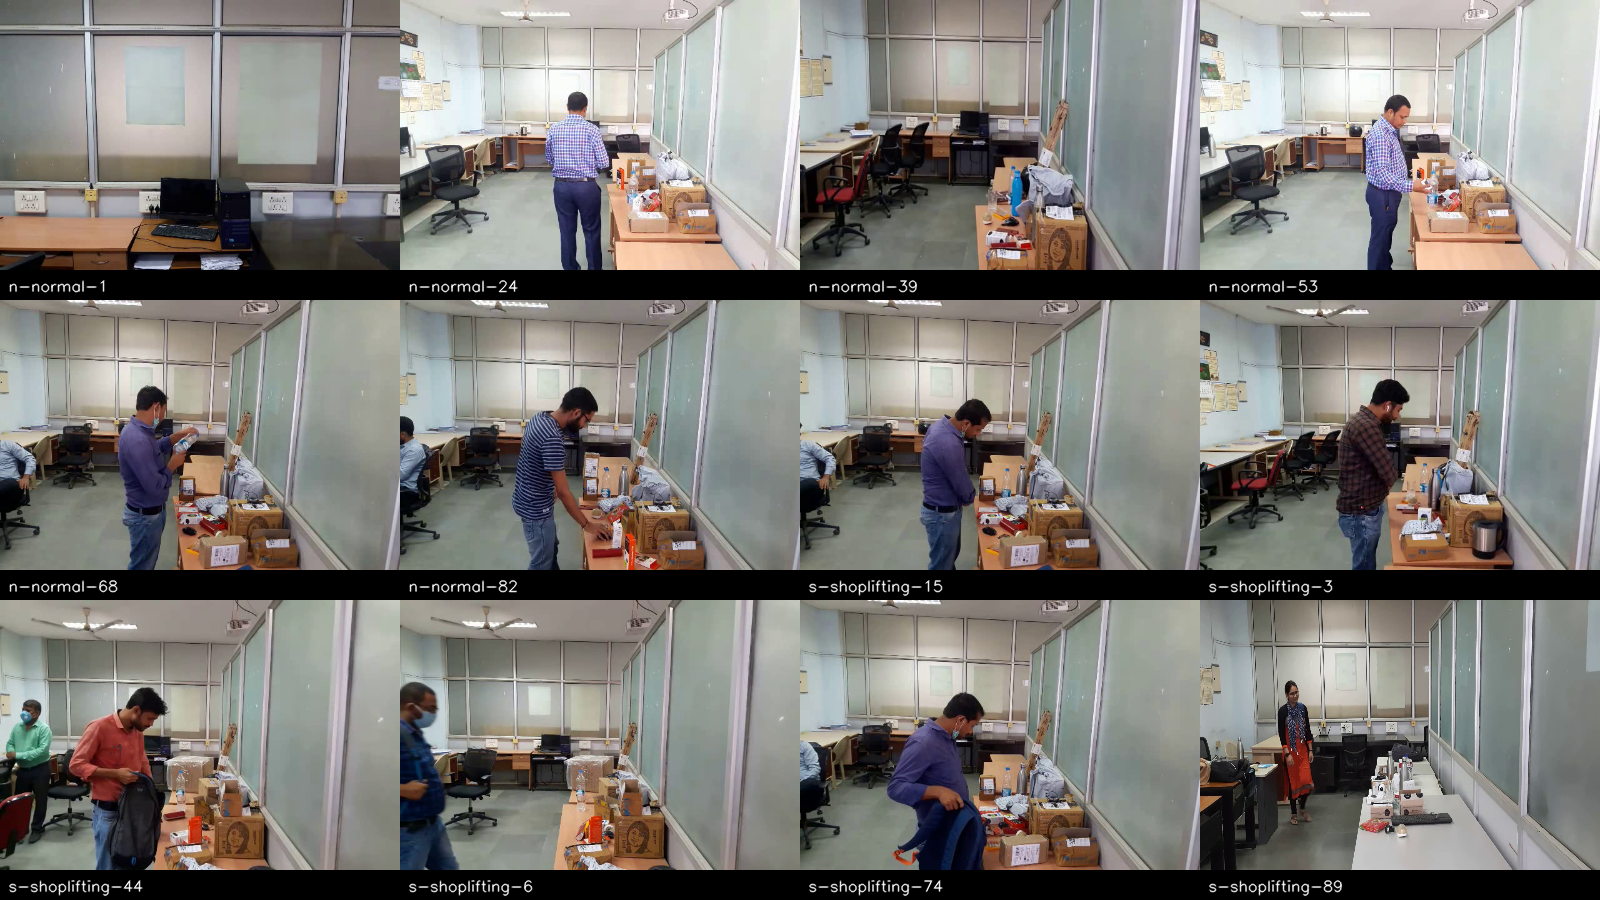
\includegraphics[width=\textwidth]{imagenes/corpus_contacto.png}
  \caption{Muestra de 12 clips tomados a lo largo de todo el corpus. Los 182
           clips son \textbf{la misma sala de oficina/laboratorio}, grabada desde
           dos posiciones de cámara, con actores. No hay tienda, góndolas, caja
           ni restaurante en ningún clip.}
  \label{fig:contacto}
\end{figure}

Los 182 clips ingestados provienen de un conjunto de datos de \emph{shoplifting}.
Se etiquetaron inicialmente como \texttt{location\_type=store} a partir del
nombre del conjunto, \textbf{sin verificarlo}. Al inspeccionar los fotogramas
(figura~\ref{fig:contacto}) quedó claro que se trata de una única sala de
oficina con actores. Se corrigieron a \texttt{location\_type=other}.

Esto tiene dos consecuencias:

\begin{enumerate}[leftmargin=*]
  \item El corpus \textbf{no representa el caso de uso}. La cifra de descarte
        medida sobre él no puede presentarse como ``porcentaje de movimiento de
        un interior comercial''.
  \item La \emph{variedad deliberada} que pide el enunciado no existe. Una sola
        sala desde dos ángulos es estadísticamente más cercano a $n=1$ que a
        $n=182$, y no se arregla añadiendo más clips de la misma fuente.
\end{enumerate}

\subsection{Las tres fuentes evaluadas}
\label{sec:fuentes}

Se evaluaron los tres conjuntos de datos disponibles. \textbf{Dos de ellos sí
contienen interiores comerciales reales}, pero ninguno en un formato utilizable
por el \emph{pipeline} completo.

\begin{center}
\begin{tabular}{@{}llll@{}}
\toprule
\textbf{Conjunto} & \textbf{Contenido} & \textbf{¿Tiendas?} & \textbf{Problema} \\
\midrule
\texttt{shoplifting2} & 182 \texttt{.mp4}, 640$\times$480, 30\,fps
                      & No & Una sala de oficina \\
\texttt{archive (1)}  & 32.458 PNG, 50 secuencias
                      & \textbf{Sí} & \textbf{64$\times$64 px} \\
Roboflow COCO         & 1.006 JPG con aumento
                      & \textbf{Sí} & Orden temporal destruido \\
\bottomrule
\end{tabular}
\end{center}

\paragraph{\texttt{archive (1)} --- contenido correcto, formato inservible.}
Es el conjunto que más se acerca al enunciado: \textbf{50 secuencias de 50
locales distintos} (29 en \texttt{Train}, 21 en \texttt{Test}), con góndolas,
mostradores, cajas y ropa, y con la variedad de altura de cámara, iluminación y
densidad de personas que se pedía. Los fotogramas están muestreados de a 10
($\approx$3\,fps efectivos), lo cual sería un punto de operación aceptable.

El problema es la resolución: \textbf{los PNG son de 64$\times$64 píxeles}. Son
miniaturas derivadas para entrenar un clasificador, no video fuente. Una persona
ocupa unos 15--20 píxeles de alto.

\begin{figure}[htbp]
  \centering
  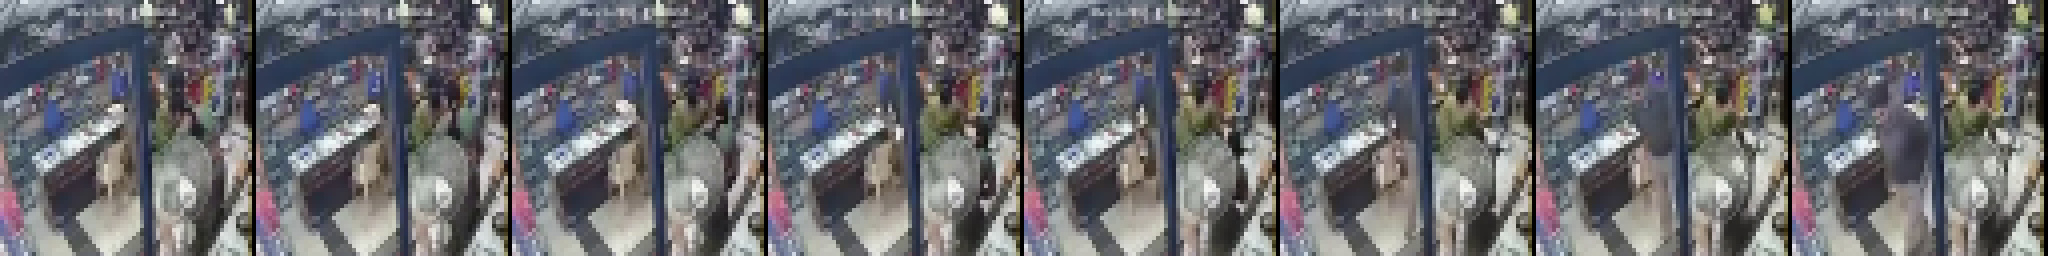
\includegraphics[width=\textwidth]{imagenes/ds_archive_nativo_x4.png}
  \caption{Ocho fotogramas consecutivos de \texttt{archive (1)}, ampliados
           4$\times$ sin interpolar. El contenido es una tienda real, pero el
           tamaño nativo de 64$\times$64 hace que una persona sea un borrón de
           unos 15 píxeles.}
  \label{fig:archivo64}
\end{figure}

Esto lo descalifica por dos motivos, y el segundo es el decisivo:

\begin{enumerate}[leftmargin=*]
  \item El Nivel~1 \emph{corre} (23,5\,\% de movimiento medido sobre la
        secuencia 003), pero sus parámetros están calibrados para 640$\times$480:
        el núcleo de apertura de 5$\times$5 representa el 7,8\,\% del ancho a
        64$\times$64, contra el 0,8\,\% a 640$\times$480. La cifra no sería
        comparable sin recalibrar.
  \item \textbf{El Nivel~2 no puede existir sobre 64$\times$64.} Ningún detector
        de objetos ni modelo visión-lenguaje produce nada útil con esa entrada.
        El \emph{pipeline} cuyo coste se quiere estimar no puede ejecutarse sobre
        este material, así que medir el Nivel~1 aquí no serviría para el objetivo
        del proyecto.
\end{enumerate}

\paragraph{Roboflow COCO --- también tiendas, pero sin orden temporal.}
La exportación reparte las imágenes aleatoriamente en \texttt{train/valid/test} y
les aplica aumento de datos. La sustracción de fondo necesita fotogramas
consecutivos del mismo plano; una colección barajada y transformada no los tiene.

\subsection{Cierre del punto 2}

Con las tres fuentes evaluadas y descartadas por motivos distintos, y sin
posibilidad de grabar en un establecimiento (sección~\ref{sec:ciclo}), el punto~2
se cierra con esta constancia:

\begin{itemize}[leftmargin=*]
  \item La \textbf{herramienta} está completa y probada: esquema, índice,
        manifest con hashes, medición de iluminación, ingesta y reetiquetado.
        Ingiere cualquier corpus futuro sin cambios.
  \item El \textbf{material disponible} se evaluó exhaustivamente. Existe metraje
        comercial real, pero sólo en formatos derivados que no sirven para el
        \emph{pipeline} completo.
  \item La \textbf{consecuencia} se arrastra explícitamente a todos los
        resultados: la tasa de descarte medida se reporta siempre con su alcance,
        y la cifra transferible se obtiene por composición de regímenes
        (sección~\ref{sec:ciclo}), no por medición directa sobre el corpus.
\end{itemize}

% ===========================================================================
\section{Punto 3 --- Nivel 1 de la cascada \ok}

\subsection{Qué se pedía}
Detección de movimiento sobre el flujo, midiendo qué porcentaje de fotogramas se
descarta.

\subsection{Implementación}

\texttt{detector.py} implementa sustracción de fondo MOG2 con tres guardas:

\begin{center}
\begin{tabular}{@{}p{4.2cm}p{9.5cm}@{}}
\toprule
\textbf{Guarda} & \textbf{Por qué} \\
\midrule
\emph{Warmup} (30 fotogramas) &
MOG2 marca casi todo como primer plano mientras aprende el fondo. Sin excluir
esos fotogramas, el porcentaje de movimiento sale inflado. \\
\addlinespace
\emph{Flicker} (\texttt{fg\_ratio > 0,50}) &
Un cambio global de luz enciende el fotograma entero. Se clasifica como
parpadeo, no como movimiento. \\
\addlinespace
\emph{Área mínima} (\texttt{min\_area\_frac}) &
Los blobs de ruido se descartan. \\
\bottomrule
\end{tabular}
\end{center}

\subsection{Un error real: el umbral de área dependía de la resolución}

\begin{figure}[htbp]
  \centering
  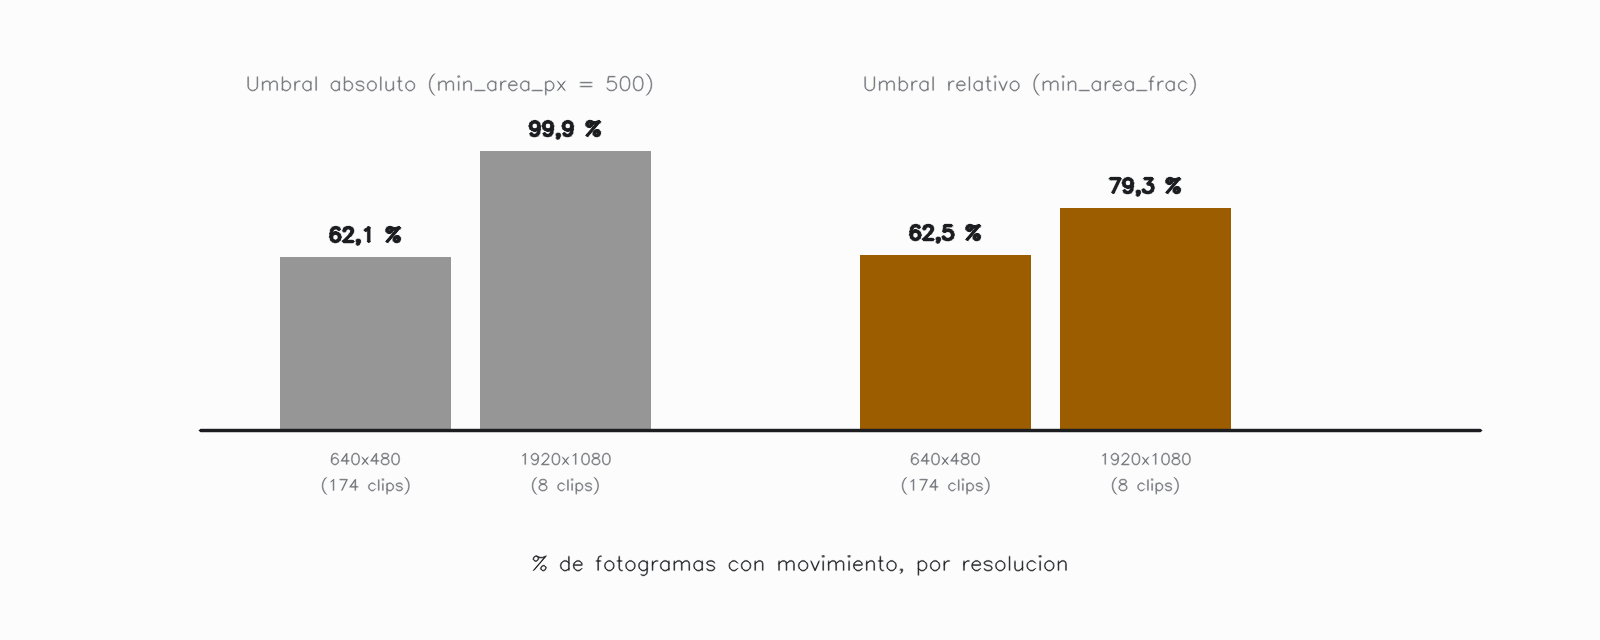
\includegraphics[width=\textwidth]{imagenes/bug_resolucion.png}
  \caption{El umbral de área era absoluto (\texttt{min\_area\_px = 500}), lo que
           a 1080p resulta 6,75 veces más sensible que a 480p. Los ocho clips de
           1920$\times$1080 reportaban 99,9\% de movimiento frente al 62,1\% de
           los 174 clips de 640$\times$480 --- por la resolución, no por el
           contenido. Con el umbral expresado como fracción del área del
           fotograma, el sesgo desaparece.}
  \label{fig:bugres}
\end{figure}

Un corpus de resolución mixta producía resultados incomparables. La corrección
consiste en expresar el umbral como fracción del área del fotograma
(\texttt{min\_area\_frac = 0,0016}, equivalente a los mismos 500\,px en
640$\times$480). Existe un test de regresión que ejecuta la misma escena
sintética a ambas resoluciones y exige el mismo veredicto.

\subsection{Resultado}

\begin{figure}[htbp]
  \centering
  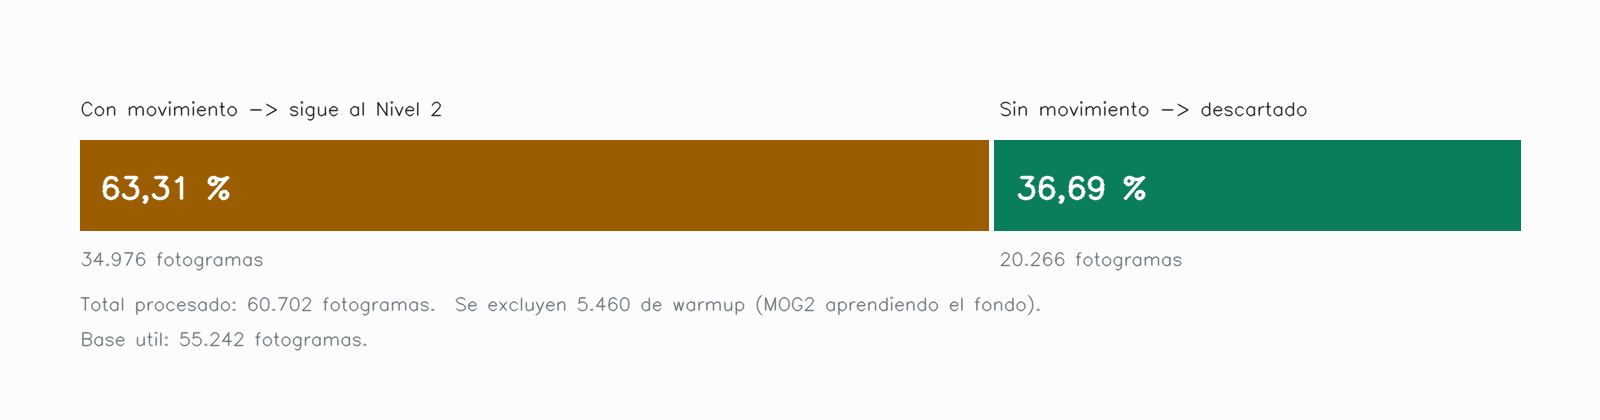
\includegraphics[width=\textwidth]{imagenes/presupuesto_frames.png}
  \caption{Reparto de los fotogramas del corpus. De 60.702 procesados, 5.460 son
           de \emph{warmup} y se excluyen; de los 55.242 útiles, 20.266
           (\dato{36,69\%}) se descartan sin coste alguno.}
  \label{fig:presupuesto}
\end{figure}

\begin{figure}[htbp]
  \centering
  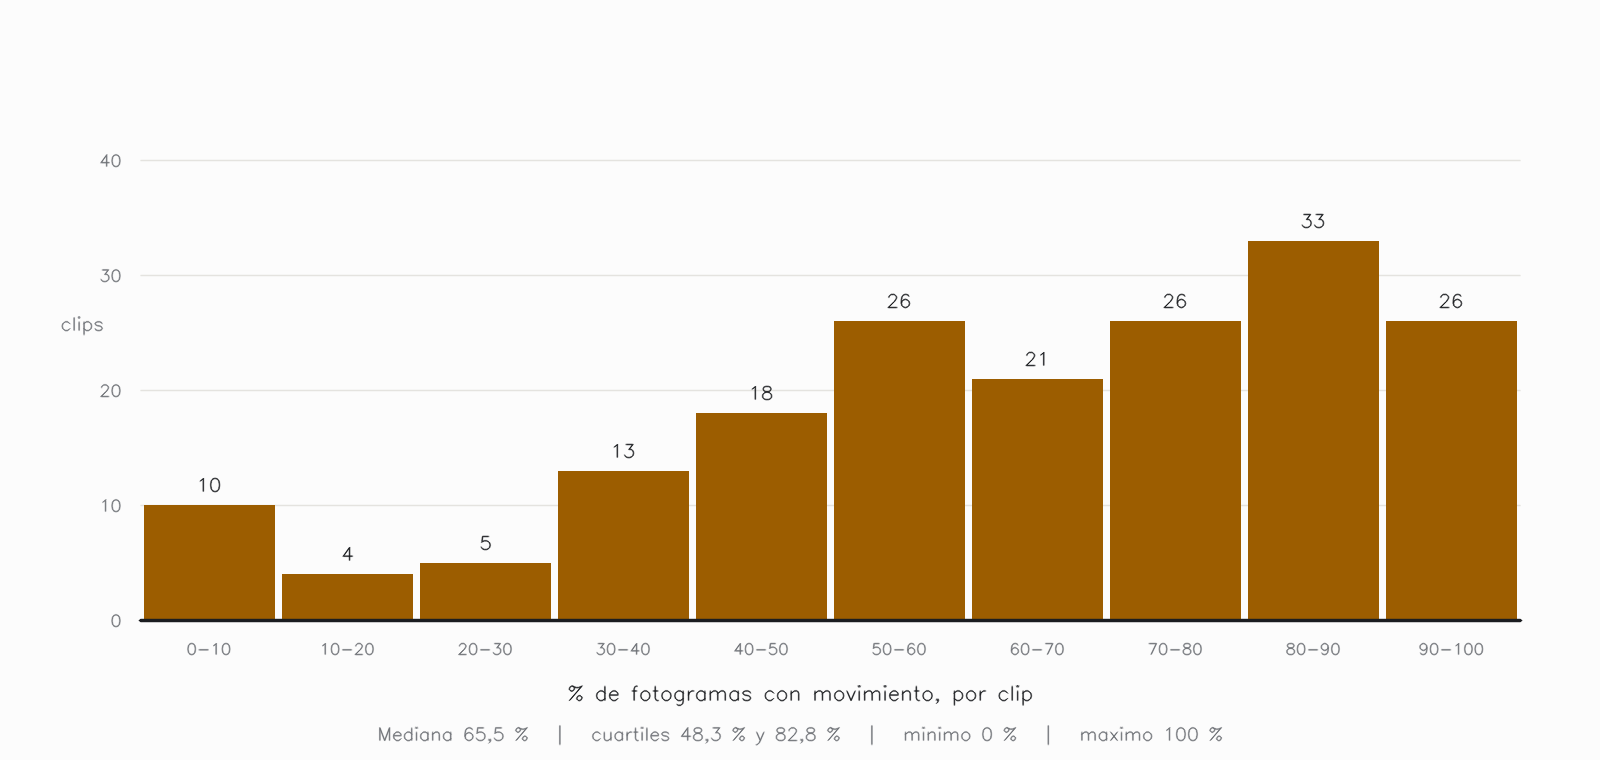
\includegraphics[width=\textwidth]{imagenes/histograma_movimiento.png}
  \caption{Distribución del porcentaje de movimiento por clip. La dispersión es
           muy amplia: hay clips que no descartan nada y clips que descartan
           todo. Un promedio único esconde esa estructura.}
  \label{fig:histograma}
\end{figure}

El Nivel~1 evita procesar el \dato{36,69\%} de los fotogramas. Es una medición
real \emph{de este corpus}, pero el corpus son clips actuados donde casi siempre
hay alguien en escena. Un comercio real está vacío de noche y en horas muertas,
por lo que el descarte verdadero sería bastante mayor.
\texttt{reporte.py} se niega a publicar la cifra como titular mientras el corpus
tenga cero clips de interior comercial.

\subsection{Una hipótesis que resultó falsa}

Los seis clips clasificados como \texttt{dim} promediaban 1,3\% de movimiento
frente al 65\% de los \texttt{bright}. La lectura obvia era que MOG2 se queda
ciego sin contraste: un falso negativo justo de noche, que habría sido un error
de corrección grave.

\begin{figure}[htbp]
  \centering
  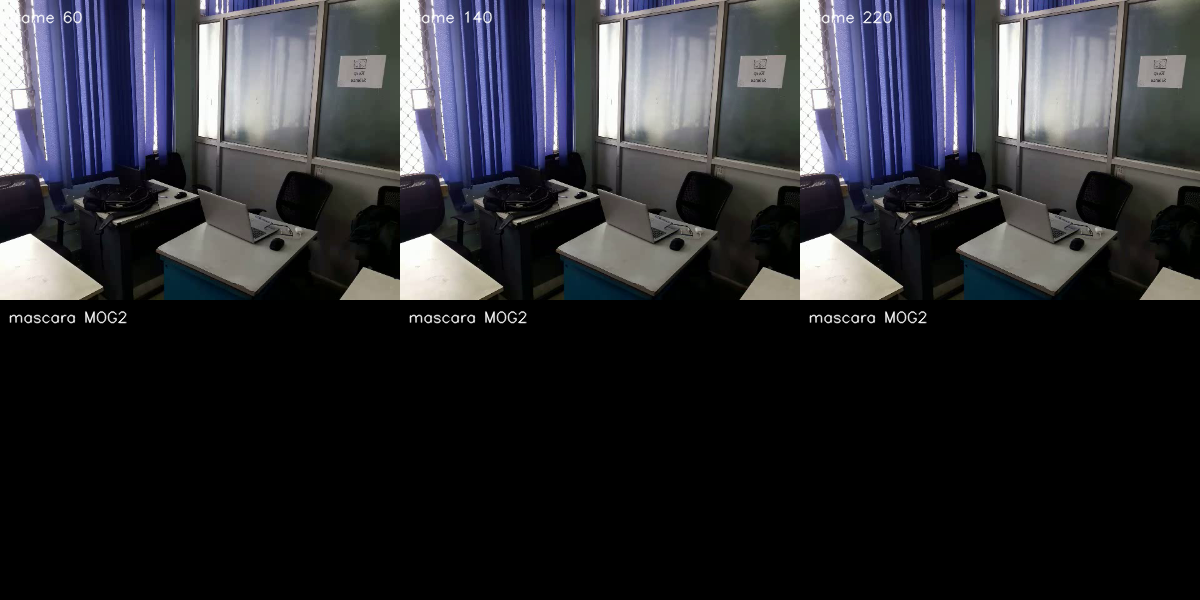
\includegraphics[width=\textwidth]{imagenes/clip_vacio.png}
  \caption{Clip \texttt{normal-13}, clasificado \texttt{dim}, con 0\% de
           movimiento. Arriba, tres fotogramas; abajo, la máscara de MOG2. La
           sala está \textbf{vacía}: no hay nadie que detectar. El Nivel~1
           acierta al descartarla.}
  \label{fig:vacio}
\end{figure}

\begin{figure}[htbp]
  \centering
  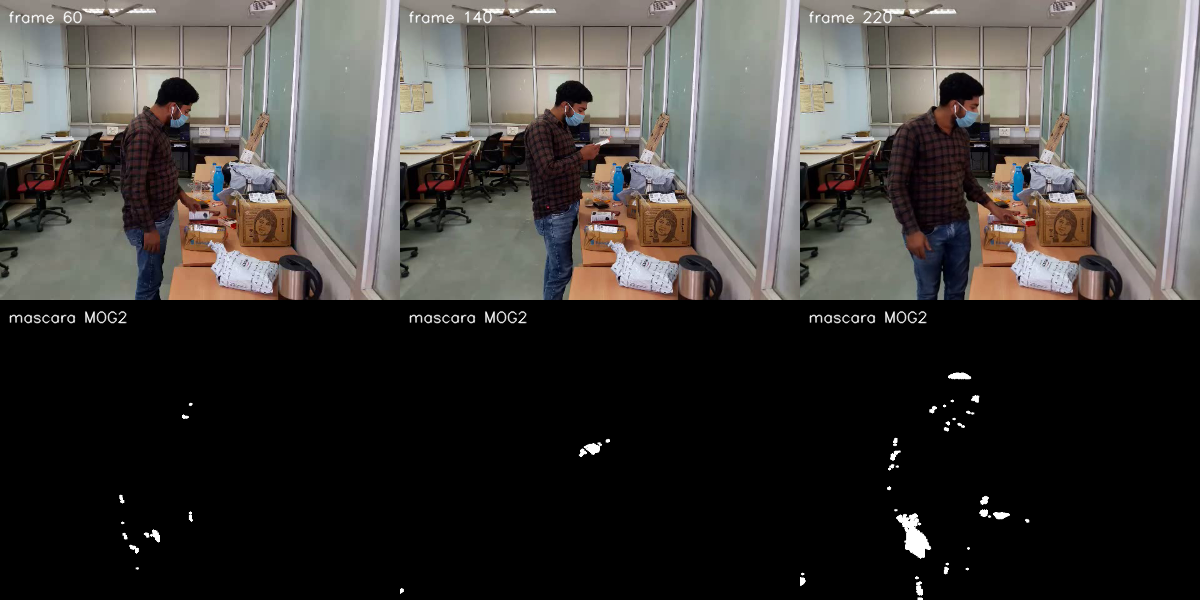
\includegraphics[width=\textwidth]{imagenes/clip_persona.png}
  \caption{Clip \texttt{normal-37}, con 83,6\% de movimiento. Hay una persona en
           escena y la máscara la recoge. El detector funciona.}
  \label{fig:persona}
\end{figure}

Al extraer los fotogramas y mirarlos (figuras~\ref{fig:vacio}
y~\ref{fig:persona}) la explicación resultó ser otra: \textbf{esas tomas son de
la sala vacía}. Se comprobó además que MOG2 sí produce primer plano en esos
clips (0,24\% de los píxeles), pero es ruido disperso del códec que la apertura
morfológica elimina, que es exactamente lo que debe hacer.

De haber ``corregido'' el detector con ecualización de contraste o un umbral más
bajo, se lo habría ajustado para alucinar movimiento en habitaciones vacías. La
pregunta sobre el comportamiento con poca luz \emph{real} y personas en escena
queda abierta: este corpus no permite responderla.

% ===========================================================================
\section{Punto 4 --- Instrumentación de coste \ok}

\subsection{Qué se pedía}
Antes que ningún modelo: un módulo que registre, por cada evento procesado, el
tiempo de CPU, el tiempo de GPU, los tokens consumidos y el coste en dólares.

\subsection{Esquema}

\begin{lstlisting}[language=SQL]
CREATE TABLE cost_events (
    event_id     TEXT PRIMARY KEY,
    run_id       TEXT NOT NULL,   -- agrupa los eventos de una corrida
    timestamp    TEXT NOT NULL,   -- ISO-8601 UTC
    stage        TEXT NOT NULL,
    cpu_time_ms  REAL NOT NULL,
    gpu_time_ms  REAL NOT NULL,   -- lo llenan las etapas GPU (semana 2+)
    tokens_used  INTEGER NOT NULL,-- lo llenan las llamadas a VLM (semana 3+)
    cost_usd     REAL NOT NULL,
    wall_time_ms REAL NOT NULL,   -- reloj de pared: incluye I/O y red
    meta         TEXT NOT NULL    -- JSON libre (n_frames, clip_id, ...)
);
\end{lstlisting}

Instrumentar cualquier etapa futura es una línea:

\begin{lstlisting}[language=Python]
with tracker.track("object_detection", clip_id=cid) as ev:
    ...
    ev.gpu_time_ms = t_gpu       # etapas GPU
    ev.tokens_used = n_tokens    # llamadas a VLM
\end{lstlisting}

\subsection{Tres decisiones de diseño}

\begin{enumerate}[leftmargin=*]
  \item \textbf{\texttt{cpu\_time\_ms} usa \texttt{time.process\_time\_ns()}} ---
        tiempo de CPU, no de reloj, para que esperar el stream RTSP no se
        facture como cómputo. Se puede comprobar que funciona: el evento del
        stream registró 13.071\,ms de CPU contra 13.787\,ms de reloj. Es una
        medida del proceso completo, así que sólo es válida en etapas
        secuenciales; si alguna etapa se paraleliza habrá que pasar a
        \texttt{time.thread\_time\_ns()} por trabajador.

  \item \textbf{Los eventos se acumulan en memoria y se escriben con
        \texttt{executemany}.} A nivel de fotograma, un \texttt{INSERT} de SQLite
        costaría más que el propio MOG2 y contaminaría la medición que se está
        tomando. Se emite un evento por clip, con \texttt{n\_frames} en
        \texttt{meta}, de modo que el coste por fotograma sigue siendo derivable.

  \item \textbf{\texttt{cost\_usd} es 0 por construcción.}
        \texttt{AMTA\_CPU\_USD\_PER\_HOUR} vale \texttt{0.0} por defecto
        deliberadamente, para que nadie cite un coste inventado. Los
        milisegundos sí son reales.
\end{enumerate}

\subsection{Un error que sólo apareció al ejecutar}

La base de datos acumula entre corridas, de modo que el reporte sumaba corridas
anteriores: 14 eventos donde debía haber 7. Se corrigió añadiendo \texttt{run\_id}
y filtrando por él, más una migración \texttt{ALTER TABLE} para bases creadas por
la versión anterior. Tiene test de regresión.

\subsection{Resultado}

\begin{center}
\begin{tabular}{@{}llll@{}}
\toprule
\textbf{Campo} & \textbf{Valor actual} & \textbf{Quién lo llena} \\
\midrule
\texttt{cpu\_time\_ms} & 4,36 -- 38,77 ms/fotograma & ya medido, real \\
\texttt{gpu\_time\_ms} & 0                          & etapas GPU, semana 2+ \\
\texttt{tokens\_used}  & 0                          & llamadas a VLM, semana 3+ \\
\texttt{cost\_usd}     & 0                          & al fijar la tarifa \\
\bottomrule
\end{tabular}
\end{center}

Medición agregada: \dato{7,28 ms de CPU por fotograma} a 640$\times$480, con un
solo hilo (\texttt{cv2.setNumThreads(1)} para que la medición sea reproducible).
Este número \emph{sí} es transferible: depende del detector y de la resolución,
no del contenido de la imagen.

% ===========================================================================
\section{El sesgo de muestreo y cómo rodearlo}
\label{sec:ciclo}

\subsection{El problema}

La duración mediana de los clips del corpus es de 11 segundos, y son segmentos
elegidos porque en ellos ocurre algo. Una cámara real graba de forma continua y
está vacía la mayor parte del tiempo: de noche, antes de abrir, en horas muertas.
El 36,69\% medido corresponde por tanto a un régimen de actividad muy alto, no al
de una jornada completa.

\subsection{Por qué no se resuelve grabando en un comercio}

La salida aparentemente obvia —poner una cámara en una tienda y grabar unas
horas— no es aceptable sin más. Grabar personas identificables en un
establecimiento implica autorización expresa del titular, señalización visible y
tratamiento de datos personales; no es algo que se pueda hacer de manera
informal para un experimento. Se descarta como tarea del proyecto.

\subsection{La vía técnica: componer el ciclo de actividad}

El corpus \emph{ya contiene} los dos regímenes, grabados por la misma cámara fija:

\begin{itemize}[leftmargin=*]
  \item \textbf{Escena vacía} --- los clips \texttt{dim} y los del primer decil
        del histograma (figura~\ref{fig:histograma}) son tomas de la sala sin
        nadie: 0\% de movimiento. Son, literalmente, metraje de ``no pasa nada''.
  \item \textbf{Escena activa} --- el resto, con una o dos personas.
\end{itemize}

Con ambos se puede construir un ciclo de actividad arbitrario y medir el descarte
sobre él. Si $f_{a}$ es la fracción del día con actividad, y $p_{a}$, $p_{v}$ son
las tasas de paso medidas en cada régimen, la tasa global es:

\[
  p \;=\; f_{a}\,p_{a} \;+\; (1-f_{a})\,p_{v}
\]

Ambos regímenes están medidos sobre el corpus:

\begin{center}
\begin{tabular}{@{}lrrr@{}}
\toprule
\textbf{Régimen} & \textbf{clips} & \textbf{fotogramas útiles} & \textbf{tasa de paso} \\
\midrule
Escena vacía  ($p_v$) &  10 &  2.916 & 0,0106 \\
Escena activa ($p_a$) & 172 & 52.326 & 0,6678 \\
\bottomrule
\end{tabular}
\end{center}

\noindent
Con esos dos valores, el descarte del Nivel~1 para distintos ciclos de actividad:

\begin{center}
\begin{tabular}{@{}rrr@{}}
\toprule
\textbf{Actividad ($f_a$)} & \textbf{Tasa de paso $p$} & \textbf{Descarte} \\
\midrule
 5\,\% &  0,0435 & 95,7\,\% \\
10\,\% &  0,0764 & 92,4\,\% \\
15\,\% &  0,1092 & \dato{89,1\,\%} \\
25\,\% &  0,1749 & 82,5\,\% \\
50\,\% &  0,3392 & 66,1\,\% \\
\midrule
\multicolumn{2}{@{}l}{\emph{corpus tal cual (sesgado)}} & 36,7\,\% \\
\bottomrule
\end{tabular}
\end{center}

\noindent
Un comercio activo el 15\% de las 24~horas daría un descarte cercano al
\dato{89\%}, no al 37\%. La diferencia es enorme y va toda en la dirección de
favorecer la cascada.

Esto convierte el metraje faltante en un \textbf{parámetro} en lugar de un
bloqueo. La proyección de coste se entrega como una superficie sobre $f_a$, y
cuando se conozca el ciclo real de un local concreto —un dato de operación, que
el propio establecimiento conoce, no algo que haya que grabar— se sustituye y se
lee el resultado.

\subsection{Alternativas legítimas si hiciera falta metraje continuo}

\begin{itemize}[leftmargin=*]
  \item \textbf{Las propias instalaciones de AMTA}: una cámara fija en un pasillo
        o sala del laboratorio, con el personal informado. Es espacio propio y
        gente del equipo; reproduce el patrón de ocupación intermitente que
        interesa medir.
  \item \textbf{Conjuntos de datos públicos con grabación continua} y licencia
        que permita el uso, si se encuentra alguno. La mayoría de los conjuntos
        de videovigilancia publicados vienen recortados por eventos, que es
        precisamente el sesgo que se quiere evitar.
  \item \textbf{Un acuerdo formal con un establecimiento}, con autorización
        escrita y señalización. Es la vía correcta, pero es un trámite de
        negocio, no una tarea de ingeniería.
\end{itemize}

% ===========================================================================
\section{El punto de equilibrio de la cascada}

Hay un resultado que no depende del corpus y que conviene conocer antes de
construir el Nivel~2.

El Nivel~1 se ejecuta sobre el \textbf{100\%} de los fotogramas, pero sólo evita
la fracción descartada del trabajo del Nivel~2. La cascada se paga si y sólo si:

\[
  C_{1} \;<\; (1 - p)\cdot C_{2}
  \qquad\Longrightarrow\qquad
  C_{2} \;>\; \frac{C_{1}}{1-p}
\]

\noindent
donde $C_1$ y $C_2$ son los costes por fotograma de cada nivel y $p$ es la
fracción de fotogramas que pasan el filtro. Con los valores medidos
($C_1 = 7{,}28$\,ms, $p = 0{,}6331$):

\[
  C_{2} \;>\; \frac{7{,}28}{0{,}3669} \;\approx\; 19{,}8\ \mathrm{ms/fotograma}
\]

\noindent
Es decir: con la tasa de paso sesgada del corpus, \dato{el Nivel~2 debería costar
más de 19,8\,ms por fotograma} para que la cascada tenga sentido.

Pero esa cifra es la peor posible, porque $p$ está inflado por el sesgo de
muestreo. Con el ciclo de actividad de la sección~\ref{sec:ciclo}, el umbral cae
mucho:

\begin{center}
\begin{tabular}{@{}rrr@{}}
\toprule
\textbf{Actividad ($f_a$)} & \textbf{$p$} & \textbf{$C_2$ mínimo para que compense} \\
\midrule
10\,\% & 0,0764 & 7,9\ ms/fotograma \\
15\,\% & 0,1092 & \dato{8,2\ ms/fotograma} \\
25\,\% & 0,1749 & 8,8\ ms/fotograma \\
50\,\% & 0,3392 & 11,0\ ms/fotograma \\
\midrule
\multicolumn{2}{@{}l}{\emph{corpus tal cual}} & 19,8\ ms/fotograma \\
\bottomrule
\end{tabular}
\end{center}

\noindent
En un escenario realista basta con que el Nivel~2 cueste algo más de
\textbf{8\,ms por fotograma} —un umbral que cualquier detector de objetos supera
holgadamente— para que la cascada se pague. La conclusión práctica es que la
arquitectura en cascada está justificada; lo que el corpus sesgado hacía era
esconder ese hecho.

Si el Nivel~2 resulta más barato que eso, el Nivel~1 es puro sobrecoste y
conviene ejecutar el Nivel~2 sobre todo. Con un corpus representativo el
descarte sería mayor, $p$ bajaría y ese umbral se relajaría --- razón adicional
para conseguir metraje real antes de dimensionar el Nivel~2.

% ===========================================================================
\section{Veredicto y trabajo pendiente}

\subsection{Estado de los cuatro puntos}

\begin{center}
\begin{tabular}{@{}clp{7.5cm}@{}}
\toprule
\textbf{\#} & \textbf{Punto} & \textbf{Estado} \\
\midrule
1 & Simulador de cámara & \ok{} Funcionando, con reconexión verificada. \\
2 & Corpus de video     & \cerrado{} Herramienta completa y probada. Las tres
                           fuentes evaluadas; ninguna utilizable (ver \S\ref{sec:fuentes}).
                           Limitación documentada y arrastrada a los resultados. \\
3 & Nivel 1             & \ok{} 36,69\% de descarte medido; motor validado. \\
4 & Instrumentación     & \ok{} 7,28 ms/fotograma; esquema completo. \\
\bottomrule
\end{tabular}
\end{center}

\subsection{Qué falta}

\begin{enumerate}[leftmargin=*]
  \item \textbf{Componer un ciclo de actividad realista} con el material que ya
        hay (sección~\ref{sec:ciclo}). Es la vía para estimar el descarte sobre
        24~horas sin grabar nada nuevo.

  \item \textbf{Fijar una tarifa de CPU verificada} y convertir los
        7,28\,ms/fotograma en dólares por cámara y mes. No depende de conseguir
        más metraje: el modelo queda parametrizado en $p$.

  \item \textbf{Probar el Nivel~1 con poca luz real}, con personas en escena.
        El corpus actual no permite responderlo; la sala propia del laboratorio
        sí lo permitiría, con luz apagada y personal del equipo.

  \item \textbf{Verificar \texttt{crowd\_density}.} Los 182 clips están
        etiquetados \texttt{sparse} por defecto, con una nota que lo indica. Es
        el único eje que no se pudo medir; se resolverá cuando el Nivel~2 cuente
        personas.
\end{enumerate}

\subsection{Reproducir los resultados}

\begin{lstlisting}[language=bash]
cd v-jepa-2/docker

# 1. Construir la imagen
docker compose build cascade

# 2. Tests (34 en verde)
docker compose run --rm cascade python -m pytest tests/cascade -v

# 3. Levantar el simulador RTSP
RTSP_CLIP=<clip>.mp4 docker compose up -d mediamtx publisher

# 4. Barrido completo del corpus + medicion sobre el stream
docker compose run --rm cascade python -m core.cascade.run_stage1 --rtsp

# 5. Apagar
docker compose down
\end{lstlisting}

Salidas en \texttt{v-jepa-2/results/}: \texttt{stage1\_motion\_report.md}
(reporte legible), \texttt{stage1\_motion\_stats.json} (datos por clip) y
\texttt{costs.db} (log de coste en SQLite).

\end{document}
